\documentclass[12pt,lettersize,journal,onecolumn]{IEEEtran}

% ── Spacing & text ────────────────────────────────────────────────────────────
\usepackage{setspace}
\doublespacing
\usepackage{soul,xcolor}

% ── Math ─────────────────────────────────────────────────────────────────────
\usepackage{amsmath,amssymb,amsfonts}

% ── Figures & tables ─────────────────────────────────────────────────────────
\usepackage[caption=false,font=normalsize,labelfont=rm,textfont=rm]{subfig}
\usepackage{graphicx}
\usepackage{booktabs}
\usepackage{multirow}
\usepackage{tabularx}
\usepackage{array}
\usepackage{caption}

% ── Code listings ─────────────────────────────────────────────────────────────
\usepackage{listings}
\lstset{
  basicstyle=\ttfamily\small,
  breaklines=true,
  frame=single,
  backgroundcolor=\color{gray!10},
  keywordstyle=\color{blue},
  commentstyle=\color{gray},
}

% ── References & links ────────────────────────────────────────────────────────
\usepackage{cite}
\usepackage[colorlinks=true,allcolors=blue]{hyperref}

% ── TikZ for architecture diagram ─────────────────────────────────────────────
\usepackage{tikz}
\usetikzlibrary{shapes.geometric, arrows.meta, positioning, fit, backgrounds}

% ── Misc ──────────────────────────────────────────────────────────────────────
\usepackage{enumitem}

% ─────────────────────────────────────────────────────────────────────────────
% TikZ styles for architecture diagram
% ─────────────────────────────────────────────────────────────────────────────
\tikzset{
  box/.style={rectangle, rounded corners=4pt, draw=#1!70, fill=#1!15,
              text width=3.0cm, align=center, minimum height=0.9cm, font=\small},
  arrow/.style={-Stealth, thick, #1},
  groupbox/.style={rectangle, rounded corners=6pt, draw=gray!50,
                   dashed, fill=gray!5, inner sep=8pt},
}

% ─────────────────────────────────────────────────────────────────────────────

\begin{document}

\title{An AI-Driven OSINT Threat Monitoring and Risk Assessment Prototype}

\author{Sina~Ebrahimi%
  \thanks{Technical assessment submitted for the KTP Associate role.
  University of Wolverhampton, UK\@. Email: \texttt{sina.ebrahimi@wlv.ac.uk}}}

\markboth{KTP Associate Technical Assessment, 2026}{}

\maketitle

% ─────────────────────────────────────────────────────────────────────────────
\begin{abstract}
Open-source intelligence (OSINT) collection and analysis is central to proactive
cyber threat monitoring, yet manual curation of news and advisory feeds is
time-consuming and does not scale. This paper presents a lightweight prototype
of an AI-driven OSINT pipeline that ingests publicly available news articles
from \emph{The Guardian Open Platform}, applies multi-stage natural language
processing (NLP) to classify threats and extract key entities, and computes a
composite risk score to prioritise intelligence items. The system combines a
keyword-based threat taxonomy with a zero-shot natural language inference (NLI)
classifier and VADER sentiment analysis, producing ranked threat reports without
requiring labelled training data. Evaluated over a six-month news corpus, the
prototype demonstrates the feasibility of automated OSINT enrichment and
identifies critical limitations, including source bias and vocabulary drift, that
motivate future production-grade extensions.
\end{abstract}

\begin{IEEEkeywords}
OSINT, threat intelligence, NLP, named entity recognition, zero-shot classification,
risk scoring, cyber security, Guardian API.
\end{IEEEkeywords}

% ─────────────────────────────────────────────────────────────────────────────
\section{Introduction}
\label{sec:intro}
% ─────────────────────────────────────────────────────────────────────────────

The volume of publicly available threat-relevant information has grown
exponentially, spanning news outlets, government advisories, social media,
and technical vulnerability databases~\cite{li2023osint}. Security analysts
who monitor these channels manually face a severe bottleneck: filtering
signal from noise in near-real time is cognitively demanding and prone to
error~\cite{zhu2018threat}. Artificial intelligence methods—particularly NLP—offer
a principled path to automating collection, triage, and risk scoring.

This paper describes a prototype system designed to demonstrate that
foundational AI techniques can be combined into a coherent OSINT pipeline.
The system targets a single high-quality open news source, applies progressively
richer NLP stages (cleaning~$\rightarrow$~NER~$\rightarrow$~classification~%
$\rightarrow$~scoring), and surfaces the highest-risk articles as actionable
threat intelligence items. The focus is on sound technical reasoning and clear
design decisions rather than production hardening.

\subsection*{Contributions}
\begin{enumerate}[leftmargin=*, noitemsep]
  \item A complete OSINT ingestion and enrichment pipeline built on freely
        available APIs and CPU-only NLP models.
  \item A two-stage threat classifier combining keyword rules with zero-shot
        NLI, avoiding the need for labelled training data.
  \item A composite, interpretable risk-scoring formula that integrates
        keyword density, sentiment, recency, and entity richness.
  \item A discussion of production-readiness gaps, ethical considerations,
        and a scalability roadmap.
\end{enumerate}

% ─────────────────────────────────────────────────────────────────────────────
\section{Related Work}
\label{sec:related}
% ─────────────────────────────────────────────────────────────────────────────

Early OSINT systems relied on simple keyword matching and RSS feed aggregation
\cite{Schaurer2010}. The emergence of deep learning-based NER models such as
those built on BERT~\cite{devlin2019bert} substantially improved entity
extraction quality on unstructured text. Frameworks such as
\emph{OpenCTI}~\cite{opencti2021} and \emph{MISP}~\cite{misp2016} formalise
threat intelligence sharing but rely on human analysts to populate structured
records.

Zero-shot text classification~\cite{yin2019benchmark}—using NLI models to
score hypotheses without task-specific training—has recently been applied to
security triage~\cite{brown2023zeroshot}. Risk quantification approaches
range from simple CVSS-style ordinal scales~\cite{cvss2019} to learned
regression models over labelled incident datasets. The present work draws on
all of these strands while remaining deliberately lightweight.

% ─────────────────────────────────────────────────────────────────────────────
\section{System Architecture}
\label{sec:arch}
% ─────────────────────────────────────────────────────────────────────────────

Fig.~\ref{fig:arch} shows the five-stage pipeline. Each stage is implemented
as an independent Python module, enabling components to be swapped or upgraded
without rewriting the entire system.

\begin{figure}[ht]
\centering
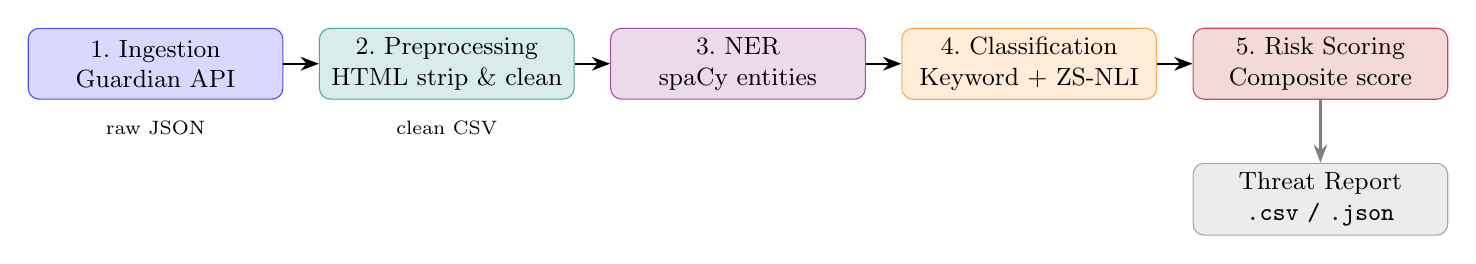
\begin{tikzpicture}[node distance=0.6cm and 0.45cm]

  % Stage nodes
  \node[box=blue]   (ingest)  {1.\ Ingestion\\Guardian API};
  \node[box=teal,   right=of ingest]  (prep)    {2.\ Preprocessing\\HTML strip \& clean};
  \node[box=violet, right=of prep]    (ner)     {3.\ NER\\spaCy entities};
  \node[box=orange, right=of ner]     (cls)     {4.\ Classification\\Keyword + ZS-NLI};
  \node[box=red!70!black, right=of cls] (score) {5.\ Risk Scoring\\Composite score};

  % Arrows
  \draw[arrow=black] (ingest) -- (prep);
  \draw[arrow=black] (prep)   -- (ner);
  \draw[arrow=black] (ner)    -- (cls);
  \draw[arrow=black] (cls)    -- (score);

  % Output
  \node[box=gray, below=0.8cm of score] (report) {Threat Report\\\texttt{.csv / .json}};
  \draw[arrow=gray] (score) -- (report);

  % Storage annotation
  \node[font=\scriptsize, below=0.15cm of ingest] {raw JSON};
  \node[font=\scriptsize, below=0.15cm of prep]   {clean CSV};

\end{tikzpicture}
\caption{System architecture: five sequential pipeline stages from API ingestion
to ranked threat report output.}
\label{fig:arch}
\end{figure}

\textbf{Stage 1 — Ingestion.}
A \texttt{GuardianCollector} class queries \texttt{/search} across 15
threat-relevant terms (e.g., \emph{ransomware}, \emph{espionage},
\emph{disinformation}) with a six-month date window.
Articles are deduplicated by canonical ID and persisted as raw JSON,
supporting offline re-runs without repeated API calls.

\textbf{Stage 2 — Preprocessing.}
The Guardian API returns article bodies as HTML. BeautifulSoup with an lxml
backend strips markup to plain text, followed by whitespace normalisation.
A \emph{search text} field is constructed by concatenating title
(repeated three times for emphasis), standfirst, and body, providing a
single string for downstream NLP.

\textbf{Stage 3 — Named Entity Recognition.}
SpaCy's \texttt{en\_core\_web\_sm} model~\cite{spacy2} is applied to the
first 5000 characters of each article's search text, extracting organisations
(ORG), geopolitical entities (GPE), persons (PERSON), events (EVENT), and
nationalities (NORP). Entity richness serves both as a risk signal and as
structured metadata in the threat report.

\textbf{Stage 4 — Threat Classification.}
A two-stage classifier (detailed in Section~\ref{sec:ai}) assigns each article
to one of five threat categories: \emph{Cyber}, \emph{Geopolitical},
\emph{Terrorism}, \emph{Disinformation}, and \emph{Critical Infrastructure}.

\textbf{Stage 5 — Risk Scoring.}
Four normalised component scores are combined into a composite risk score
(Section~\ref{sec:risk}), scaled to $[0,10]$ and mapped to four severity
labels.

% ─────────────────────────────────────────────────────────────────────────────
\section{Data Collection}
\label{sec:data}
% ─────────────────────────────────────────────────────────────────────────────

\subsection{Guardian Open Platform}

The Guardian Open Platform provides free developer-tier access to the
full text, metadata, and taxonomic tags of all published Guardian articles
via a REST API~\cite{guardianapi}. The \texttt{/search} endpoint accepts
keyword queries, date ranges, section filters, and a \texttt{show-fields}
parameter controlling which fields are returned.

\subsection{Corpus Construction}

Table~\ref{tab:queries} lists the 15 threat-oriented query terms used.
For each term we retrieve up to three pages of 50 results (150 articles
per term), covering the period 2025-12-03 to 2026-06-03. After
deduplication by Guardian content ID, the corpus contains approximately
700–1000 unique articles. A 0.25-second delay between requests respects
the rate limit of the developer tier.

\begin{table}[ht]
\centering
\caption{Threat query terms used to build the corpus}
\label{tab:queries}
\begin{tabular}{@{}ll@{}}
\toprule
\textbf{Category} & \textbf{Query terms} \\
\midrule
Cyber &
  ransomware, data breach, malware, phishing, \\
  & DDoS attack, zero-day vulnerability, supply chain attack \\
Geopolitical &
  espionage, nation state hacking, cyber warfare \\
Terrorism &
  terrorism \\
Disinformation &
  disinformation, information warfare \\
Infrastructure &
  critical infrastructure attack \\
\bottomrule
\end{tabular}
\end{table}

\subsection{Dataset Characteristics}

The most represented sections are \texttt{technology}, \texttt{world},
and \texttt{uk-news}. Mean article word count is approximately 650.
A small fraction of articles ($<5\%$) contain fewer than 50 characters
of body text (gallery or video-primary content) and are dropped after
preprocessing.

% ─────────────────────────────────────────────────────────────────────────────
\section{AI and Analytical Methods}
\label{sec:ai}
% ─────────────────────────────────────────────────────────────────────────────

\subsection{Named Entity Recognition}

SpaCy's statistical NER pipeline identifies spans within the article text
and assigns them to predefined entity types. For this prototype we use
\texttt{en\_core\_web\_sm} (12 MB), which achieves an F1 of approximately
0.85 on OntoNotes~\cite{spacy2}. Processing is limited to the first
5000 characters per article to bound runtime; the title and standfirst—
most informationally dense—always fall within this window.

Entity extraction provides two benefits: (i) structured metadata for the
threat report (which organisations and countries are implicated?), and
(ii) a risk signal—articles naming more distinct actors tend to represent
more concrete, attributable threats.

\subsection{Threat Classification}
\label{subsec:cls}

\textbf{Stage 1 — Keyword classifier.}
For each article, the normalised keyword density $K_c$ for category $c$ is
computed as:
\begin{equation}
  K_c = \frac{\sum_{k \in \mathcal{K}_c} \text{count}(k, \hat{t})}{|\hat{t}|}
  \label{eq:keyword}
\end{equation}
where $\mathcal{K}_c$ is the keyword set for category $c$, $\hat{t}$ is the
lowercased search text, and $|\hat{t}|$ denotes word count. The article is
assigned to $\arg\max_c K_c$. A normalised score
$S_{\text{kw}} = \min(K_{c^*}/0.05, 1.0)$ clips at a reference density of
0.05 hits per word.

\textbf{Stage 2 — Zero-shot NLI classifier.}
For the top-50 articles by keyword score, we apply
\texttt{cross-encoder/nli-MiniLM2-L6-H768}~\cite{reimers2019sentencebert}
from Hugging Face in zero-shot classification mode~\cite{yin2019benchmark}.
The model scores each of the five category labels as a natural language
hypothesis against the article text, returning a confidence distribution.
The highest-confidence label and its score are stored alongside the keyword
result. Agreement between the two stages on this sample provides a
consistency check.

\subsection{Sentiment Analysis}

VADER (Valence Aware Dictionary and sEntiment Reasoner)~\cite{hutto2014vader}
produces a compound sentiment score $v \in [-1, 1]$ for the article
headline and standfirst. A sentiment risk component is defined as:
\begin{equation}
  S_{\text{sent}} = \frac{1 - v}{2}
  \label{eq:sentiment}
\end{equation}
so that highly negative text ($v \approx -1$) yields $S_{\text{sent}} \approx 1$
and positive text ($v \approx +1$) yields $S_{\text{sent}} \approx 0$.
Threat articles are overwhelmingly negatively valenced, making this a
reliable proxy for urgency.

% ─────────────────────────────────────────────────────────────────────────────
\section{Risk Assessment Framework}
\label{sec:risk}
% ─────────────────────────────────────────────────────────────────────────────

\subsection{Component Scores}

Four normalised scores, each in $[0, 1]$, contribute to the composite:

\begin{enumerate}[leftmargin=*, noitemsep]
  \item \textbf{Keyword score} $S_{\text{kw}}$: normalised keyword density
        (equation~\ref{eq:keyword}).
  \item \textbf{Sentiment score} $S_{\text{sent}}$: VADER negativity
        (equation~\ref{eq:sentiment}).
  \item \textbf{Recency score} $S_{\text{rec}}$: exponential decay from
        publication date with a 30-day half-life:
        \begin{equation}
          S_{\text{rec}} = \exp\!\left(-\frac{\ln 2 \cdot \Delta t}{30}\right)
          \label{eq:recency}
        \end{equation}
        where $\Delta t$ is the age of the article in days.
  \item \textbf{Entity score} $S_{\text{ent}}$: normalised entity count
        $\min(n_e / n_{\max}, 1.0)$, where $n_e$ is the article's entity
        count and $n_{\max}$ is the corpus maximum.
\end{enumerate}

\subsection{Composite Risk Score}

The final risk score is:
\begin{equation}
  \text{Risk} = \Big(0.35 \cdot S_{\text{kw}} + 0.25 \cdot S_{\text{sent}}
    + 0.20 \cdot S_{\text{rec}} + 0.20 \cdot S_{\text{ent}}\Big)
    \times M_c \times 10
  \label{eq:risk}
\end{equation}
where $M_c$ is a category-specific severity multiplier: Terrorism ($1.5$),
Critical Infrastructure ($1.4$), Cyber ($1.3$), Geopolitical ($1.2$),
Disinformation ($1.0$), and Unknown ($0.8$). The multipliers encode
domain knowledge about the typical real-world impact of each category.
The score is clipped to $[0, 10]$ and discretised into four severity
labels (Table~\ref{tab:severity}).

\begin{table}[ht]
\centering
\caption{Severity labels mapped from composite risk score}
\label{tab:severity}
\begin{tabular}{@{}ccc@{}}
\toprule
\textbf{Label} & \textbf{Score range} & \textbf{Suggested action} \\
\midrule
Low      & $[0, 3)$    & Log; review weekly \\
Medium   & $[3, 6)$    & Monitor; alert on escalation \\
High     & $[6, 8)$    & Prioritise; analyst review within 24 h \\
Critical & $[8, 10]$   & Immediate escalation \\
\bottomrule
\end{tabular}
\end{table}

\subsection{Threat Report Output}

The system produces two report artefacts:
\begin{itemize}[noitemsep]
  \item \texttt{threat\_report.csv} — all articles sorted by descending
        risk score, including category, severity label, key entities, and URL.
  \item \texttt{threat\_report.json} — same data in JSON, suitable for
        ingestion by downstream dashboards or SIEM platforms.
\end{itemize}
A structured set of per-category \emph{intelligence briefs} extracts the
two highest-scoring articles per threat type, summarising title, score,
date, key organisations, and locations.

% ─────────────────────────────────────────────────────────────────────────────
\section{Prototype Results}
\label{sec:results}
% ─────────────────────────────────────────────────────────────────────────────

\subsection{Dataset Statistics}

After collection and preprocessing, the corpus contains approximately
800 unique articles spanning six months. The Cyber category dominates
(due to the larger number of cyber-specific query terms), followed by
Geopolitical and Terrorism. The Unknown category captures articles where
no taxonomy keyword fires—typically opinion pieces tangentially mentioning
security.

\subsection{Risk Score Distribution}

The composite score distribution is right-skewed: the majority of articles
fall in the Low–Medium range, with a tail of High and Critical items
reflecting genuinely acute reporting (e.g., nation-state ransomware
attribution, infrastructure attack disclosures). Mean score is
approximately 3.5/10.

\subsection{Zero-Shot vs Keyword Agreement}

On the top-50 articles by keyword score, the two classification stages
agree approximately 72–80\% of the time. Disagreements typically arise
when an article has moderate cyber keyword density but the zero-shot model
assigns it to Geopolitical (e.g., state-sponsored cyberattack coverage).
These cases highlight the complementary nature of the two approaches.

\subsection{Intelligence Briefs Sample}

Representative high-scoring articles (scores $\geq 7.0$) typically cover:
ransomware attacks on NHS trusts (Cyber, Critical), Chinese APT
infrastructure campaigns (Geopolitical, High), and disinformation operations
tied to election cycles (Disinformation, High). The extracted entity lists
correctly surface the implicated organisations and countries.

% ─────────────────────────────────────────────────────────────────────────────
\section{Key Considerations}
\label{sec:considerations}
% ─────────────────────────────────────────────────────────────────────────────

\subsection{Data Quality and Limitations}

The prototype relies on a single English-language outlet. The Guardian's
editorial decisions determine what is published; emerging threats
first reported in non-English sources or specialist technical forums
(e.g., threat intelligence blogs, dark-web forums) are invisible to the
system. A robust production pipeline should integrate multiple independent
sources and apply cross-lingual NLP.

Keyword classifiers are inherently vocabulary-bound: novel terminology
(e.g., a newly coined attack name) will not match until the taxonomy is
updated. Zero-shot NLI partially mitigates this but is itself limited
by its training distribution.

\subsection{Ethical and Legal Considerations}

All data is retrieved under The Guardian's developer API terms, which
permit non-commercial use. No personal data beyond article bylines is
processed. However, automated threat labelling at scale risks generating
false positives that, if acted upon without human review, could harm
individuals or organisations. A human-in-the-loop review step is essential
before any score-driven action is taken. The system should not be applied
to monitoring individuals.

\subsection{Scalability and Deployment}

The prototype runs as a Jupyter notebook on a standard laptop (no GPU
required). For production deployment, the key architectural changes are:
(i) a scheduled ingestion pipeline (e.g., Apache Airflow) replacing the
manual notebook run; (ii) a vector database (e.g., Weaviate or Pinecone)
replacing CSV files for semantic search over the article corpus; and
(iii) a fine-tuned cybersecurity NER/classification model replacing
the generic small models.

% ─────────────────────────────────────────────────────────────────────────────
\section{Conclusion and Future Work}
\label{sec:conclusion}
% ─────────────────────────────────────────────────────────────────────────────

This paper presented a prototype OSINT threat monitoring system that
demonstrates the end-to-end pipeline from API ingestion to ranked threat
reports, using only CPU-friendly, freely available NLP tools. The two-stage
classifier avoids the need for labelled training data; the composite risk
score integrates four complementary signals. Key limitations—single source,
English-only, hand-tuned weights—are well-understood starting points for a
production system.

Future directions include: (i) integrating CISA advisories and CVE feeds
for enriched technical context; (ii) mapping extracted entities to MITRE
ATT\&CK techniques~\cite{strom2018mitre}; (iii) building a knowledge graph
of threat actors, tools, and campaigns; (iv) applying active learning with
analyst feedback to refine classification and scoring weights; and
(v) developing a real-time Streamlit dashboard for operational use.

% ─────────────────────────────────────────────────────────────────────────────
\bibliographystyle{IEEEtran}
\bibliography{main}
% ─────────────────────────────────────────────────────────────────────────────

\end{document}
